\section{Evolutionary Algorithm}
\section{evol}
The first part of this project consisted in finding three quantities that
influence the orbit of Earth around Sun: the mass of Sun, the mass of Earth and
the speed of Earth at the perihelion, using the evolutionary algorithms
implemented in EASEA.\\

\subsection{Method}
In order to find the three physics quantities describing the system, we
performed three distinct experiences because the
sampling method does not allow us to find these three quantities
simultaneously. It is impossible to find the mass of Earth and Sun at the same
time because they are only bound in a product in Newton's law of universal
gravitation. So there are a plethora of pairs of values leading to the same
result.\\

The first step consist in sampling the Earth orbit around Sun with the real
quantities in order to obtain a list of polar coordinates of Earth in the
heliocentric referential.\\
The genom of each individual correspond to the quantity to find (the mass or
the speed) and is initialised to a value of the same order of magnitude as the
real value.\\
From one generation to another, children are created by computing the mean of
the two parents. Each individual can mutate with a given probability. This
mutation correspond to an increase or a decrease of a given percentage of its
genom. This percentage is randomly selected in a fixed interval.\\
The score is defined as the difference between the real orbit and the orbit
with the quantity found in the genoms. That is to say: the sum of the distances
between corresponding points from the two trajectories (Figure \ref{error_1}). By
doing so, the
result of the algorithm does not directly depend on the value we want to find
but rather on samples of coordinates that could have been made without knowing
the quantity.\\
We settled for weak elitism, a form of elitism that ensures the best individual
of the global population (children and parents) is conserved in the next
generation.

\begin{figure}
    \[ error = \sum_{i=0}^{n} dist(p_{i}, \hat{p_{i}}) \]
    where:
    \begin{itemize}
        \item \(n\) denotes the number of samples (typically 1024)
        \item \(p_{i}\) corresponds to the i-th sampled point on the real
              Earth's
              trajectory
        \item \(\hat{p_{i}}\) correspond to the i-th sampled point on the
              estimated
              Earth's trajectory
        \item \(dist\) is the Euclidian distance
    \end{itemize}
    \caption{Expression of the error for evolutionary algorithms}
    \label{error_1}
\end{figure}

% La première partie du sujet consistait à retrouver trois valeurs influençant l'orbite de la Terre autour du Soleil : la masse du Soleil, la masse de la Terre et la vitesse de la Terre à la périhélie en utilisant les algorithme évolutionnaires présents dans EASEA.\\
% Pour cela nous avons procédé en trois étapes distinctes car la méthode d'échantillonnage ne permet pas de retrouver les trois quantités simultanément. En effet, il n'est pas possible de retrouver la masse de la Terre et la masse du Soleil en une seule expérience car elles sont uniquement présentes dans un produit dans la formule de Newton. Il existe donc une multitude de couples de valeurs menant au même résultat.\\
% La première étape consiste à effectuer un échantillonnage avec les valeurs réelles afin d'obtenir une liste de coordonnées polaires de la Terre dans le référentiel Héliocentrique.\\
% Le génome de chaque individu correspond à la quantité à retrouver qui est initialisée à une valeur de l'ordre de grandeur attendu.\\
% D'une génération à l'autre, un individu fils correspond à la moyenne de ses deux parents et chaque individu peut muter avec une certaine probabilité. Cette mutation corrrespond à une augmentation ou une diminution d'un certain pourcentage de sa valeur.\\
% Afin de calculer le score, on procède à un nouvel échantillonnage de la position de la Terre dans le référentiel Héliocentrique avec la valeur trouvée. Dans le cas de la vitesse de la Terre à la périhélie, la vitesse trouvée est utilisée comme vitesse initiale.\\
% Le score correspond à la somme des distances entre les points des deux trajectoires ainsi obtenues. Ainsi le résultat du programme ne dépend pas directement de la valeur à trouver mais d'échantillons qui auraient pu être observés sans connaitre la quantité.\\
% Nous utilisons de l'élitisme faible, c'est à dire que le meilleur individu de la population globale (parents et enfants) est garanti d'être conservé dans la prochaine génération.

\subsection{Mass of Sun}
Using the method previously described, we managed to find the mass of the Sun
with
100\% accuracy (Figure \ref{sun_mass_1}). As we can see on Figure
\ref{sun_mass_2}, the trajectory of the Earth around the Sun slowly approach
the real world trajectory over generations.\\

The results are quite impresive given it required less than a hundred
generations with only a hundred individuals (Table \ref{sun_mass_table}).

\begin{figure}
    \begin{lstlisting}
==================================================================
SUN MASS: 1988399999999999986508702416896.000000 (real), 1988399999999999986508702416896.000000 (estimated)
SCORE: 0.000000
==================================================================
SUN MASS: 1988399999999999986508702416896.000000 (real), 2078119486984494172163593469952.000000 (estimated)
SCORE: 41697618869063.750000
==================================================================
     59          1.430s            6000            6000 0.000000000e+00 3.0e+11 3.0e+12 3.0e+13
EASEA LOG [INFO]: Seed: 1675245974
EASEA LOG [INFO]: Best fitness: 0
EASEA LOG [INFO]: Elapsed time: 1.4326
\end{lstlisting}
    \caption{Output of the EASEA program when seeking the value of Sun's mass}
    \label{sun_mass_1}
\end{figure}

\begin{table}
    \begin{tabular}{lllll}
        Number of generations   & 60    \\
        Population size         & 100   \\
        Offspring size          & 100\% \\
        Mutation probability    & 0.2   \\
        Mutation variation rate & 0.05
    \end{tabular}
    \caption{Parameters used to find the mass of Sun}
    \label{sun_mass_table}
\end{table}

\begin{figure}
    \center
    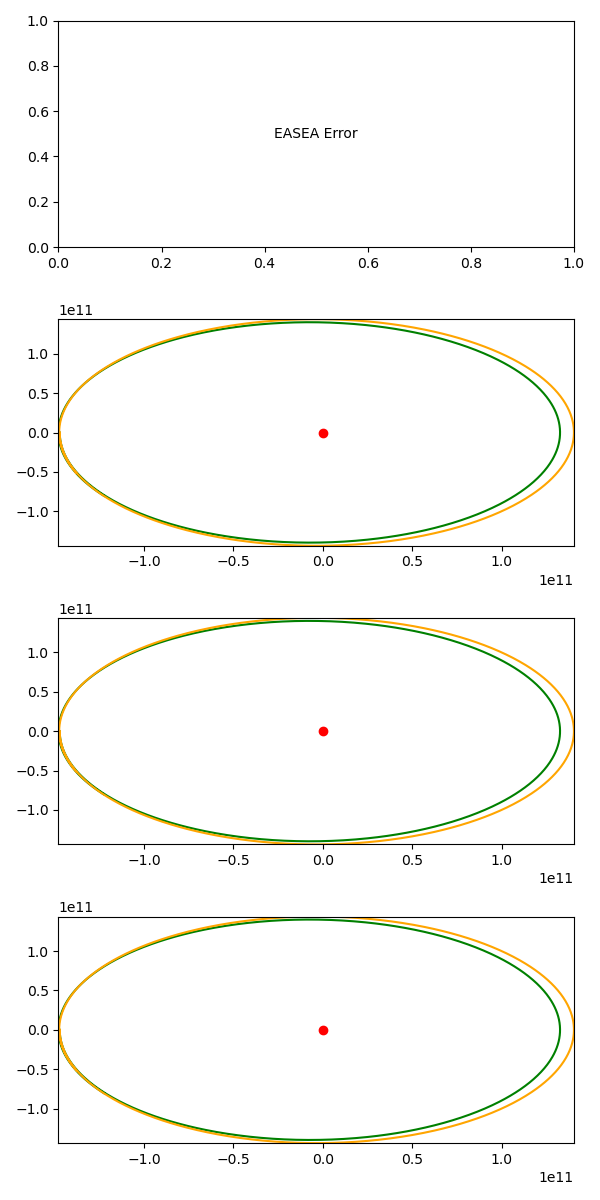
\includegraphics[scale=.3]{img/sun_mass.png}
    \caption{Earth's trajectory over generations during the evolution of Sun's
        mass}
    \label{sun_mass_2}
\end{figure}

\subsection{Mass of Earth}
We did not managed to find Earth's mass using evolutionary algorithm as this
quantity does not appear in the equations defining Earth's trajectory around
Sun. Nonetheless, we have a couple ideas regarding how we could achieve this.\\
The first being to simply change the referential: use the geocentric
referential in order to study the movement of Sun. If we only consider those
two planets (Earth and Sun) then their movements are relative to each other,
that is to say: Earth is orbiting Sun and Sun is also orbiting Earth. In that
case, we can estimate the mass of Earth exactly the same way as we did in
the previous part for the mass of Sun.\\
Another way to get to that result would be to study those two celestial bodies
in a referential centered on the center of Sun's trajectory. But in this case,
we would have to study the movement of Earth is a non-galilean referential
which is clearly out of the scope of this study.

\subsection{Speed of Earth at Perihelion}
In order to find the speed of planet Earth at the perihelion we apply the same
steps as before: initialisation, crossover, mutation and evaluation. Unless
this time we have to change a couples of values. As the speed of Earth in
radian per second is so little, it is not well handled by our program (i.e.
assimilated to zero). To combat that, we simply consider the speed in radian
per day leading to values that can properly be handled by computers. This
implies also converting the gravitationnal constant and our sampling step to
fit the new unit scale.\\

Once again, we obtained very high accuracy results (Figure \ref{speed_1}) and
we clearly see how the trajectory evolves throughout the generations (Figure
\ref{speed_2}). The results are also really impressive given the parameters we
used (Table \ref{speed_table}). The amount of generations and the population
size had to be increased compared to the first experiment, however the mutation
probability and rate are still low.\\

Playing around with the paramters reveals interesting results. On Figure
\ref{speed_low}, corresponding to a evolution with very low mutation
probability and mutation rate (typically 1\%), we clearly see that the
evolution
converges at a slower pace: there is basically no change accross the evolution
meaning the initial diversity of the population is not enough to quickly get to
the result. Increasing the mutation's paramters show significantly better
results. Figure \ref{speed_balanced} prooves that mutation generates diversity
in the population leading to a faster evolution. The two trajectories are not
yet stacked but the best individual dramatically improved during ten
generations with a really small population (5 individuals). But Figure
\ref{speed_high} shows the limits of the mutation operator. By setting a
mutation probability of 90\% and allowing a mutation to modify the individual
up to 90\%, the population struggles to converge in the right direction. The
impact of the mutation on the genome is too important, hence, we observe
oscillations: instead of approaching the real trajectory from one side, the
estimated trajectory will reach it changing side when mutation has a strong
effect.

\begin{figure}
    \begin{lstlisting}
==================================================================
PERIHELION SPEED: 0.017440 (real), 0.017440 (estimated), [1.000000]
SCORE: 0.000000
==================================================================
        99          3.397s           15000           15000 0.000000000e+00 1.6e+11 1.3e+12 1.5e+13
EASEA LOG [INFO]: Seed: 1675247174
EASEA LOG [INFO]: Best fitness: 0
EASEA LOG [INFO]: Elapsed time: 3.39933
\end{lstlisting}
    \caption{Output of the EASEA pogram when seeking the value the speed at the perihelion}
    \label{speed_1}
\end{figure}

\begin{table}
    \begin{tabular}{lllll}
        Number of generations   & 100   \\
        Population size         & 150   \\
        Offspring size          & 100\% \\
        Mutation probability    & 0.2   \\
        Mutation variation rate & 0.05
    \end{tabular}
    \caption{Parameters used to find the speed of Earth at the perihelion}
    \label{speed_table}
\end{table}

\begin{figure}
    \center
    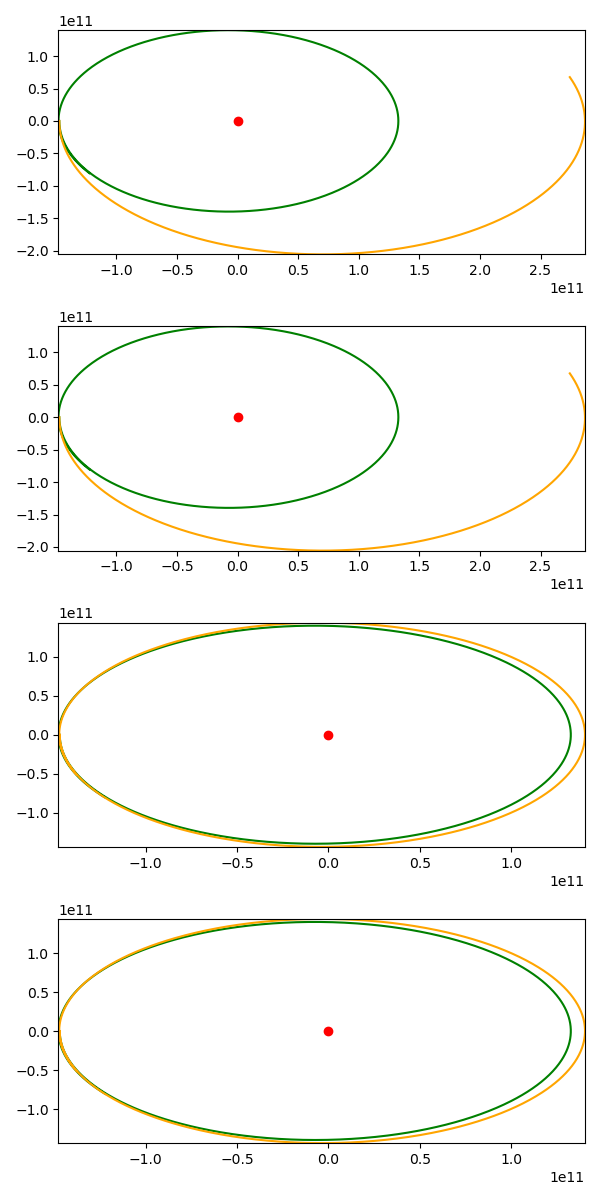
\includegraphics[scale=.3]{img/earth_speed.png}
    \caption{Earth's trajectory over generations during the evolution of
        Earth's speed at perihelion}
    \label{speed_2}
\end{figure}

\begin{figure}
    \center
    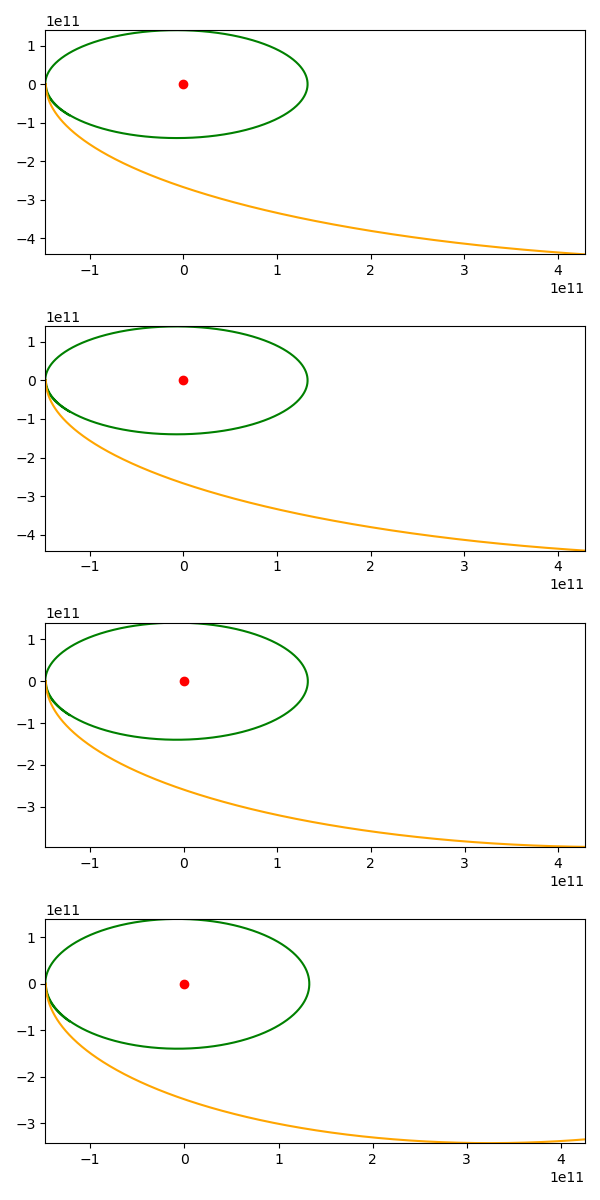
\includegraphics[scale=.3]{img/perihelion_speed_test_0.01_0.01_100_50.png}
    \caption{Earth's trajectory over generations during the evolution of
        Earth's speed at perihelion (low mutation probability and rate)}
    \label{speed_low}
\end{figure}

\begin{figure}
    \center
    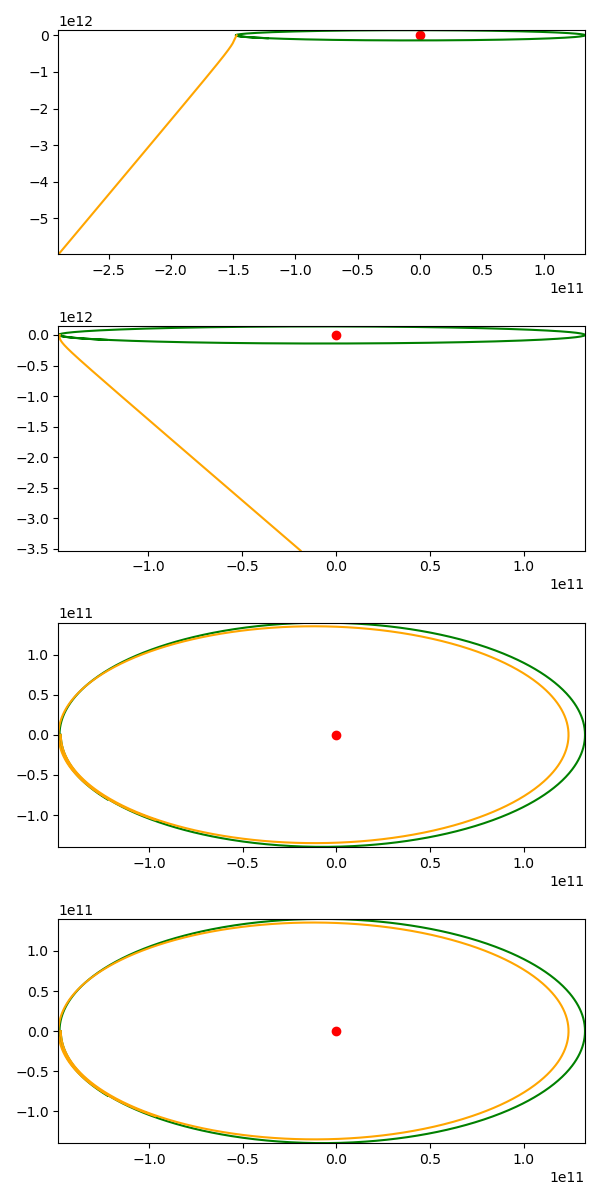
\includegraphics[scale=.3]{img/perihelion_speed_test_0.50_0.50_10_5.png}
    \caption{Earth's trajectory over generations during the evolution of
        Earth's speed at perihelion (balanced mutation probability and rate)}
    \label{speed_balanced}
\end{figure}

\begin{figure}
    \center
    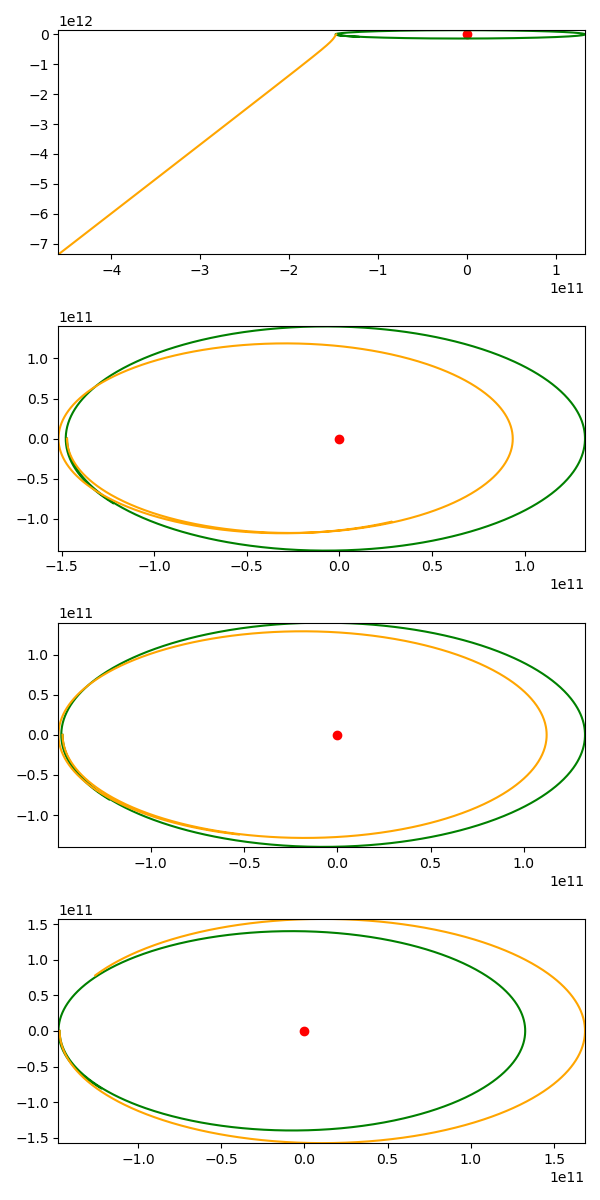
\includegraphics[scale=.3]{img/perihelion_speed_test_0.90_0.90_10_5.png}
    \caption{Earth's trajectory over generations during the evolution of
        Earth's speed at perihelion (high mutation probability and rate)}
    \label{speed_high}
\end{figure}

This part of the project demonstrates that evoltuion algorithms are very power
tools when handled properly. As long as the fitness value is meaningful and the
parameters allows the population to converge in the given amount of generations
\textemdash that is to say there is enough genetic variety (population size)
and good genetic operators (efficient mutation operator)\textemdash the output
should be close to the expected result. In this project the result structure
was simple (a single value) but in other more complex tasks the output might
look a lot different and a bit more analysis, involving a good amount of
critical thinking, must be performed in order to evaluate the correctness of
the result.